\documentclass[a4paper,11pt,twoside,notitlepage]{article}
\usepackage[left=2.5cm,right=2cm,top=2cm,bottom=2cm]{geometry}
\usepackage{graphicx}
\DeclareGraphicsExtensions{.pdf,.jpeg,.jpg}
\usepackage[colorlinks=false, pdfborder={0 0 0}]{hyperref}
\usepackage{cleveref} 
\usepackage{fancyhdr}
\usepackage{abstract}
\usepackage{framed}              %for doing nice boxes
\usepackage{amsmath}             %for math environment
\usepackage{parskip}             %for modifying spacing
\usepackage[procnames]{listings} %for inserting code
\usepackage{color}               %obv
\usepackage{appendix}            %obv
\usepackage{enumitem}            %for modifying lists
\setitemize{noitemsep,topsep=0pt,parsep=0pt,partopsep=0pt}
\setenumerate{noitemsep,topsep=0pt,parsep=0pt,partopsep=0pt}
\usepackage{float}              %for forcefully placing diagrams 
\usepackage[backref=true,
            %style=authoryear,
            style=numeric-comp,
            citereset=section,
            maxcitenames=3,
            maxbibnames=100,]{biblatex}
\bibliography{litreview}
\DefineBibliographyStrings{english}{%
    backrefpage  = {see p.}, % for single page number
    backrefpages = {see pp.} % for multiple page numbers
}
\setlength\bibitemsep{1em}
\usepackage{fancyvrb} % for inserting .txt
\usepackage{pgfplots}
\usepackage{caption} % for figures within figures
\usepackage{subcaption} %figures figures
\usepackage{adjustbox}

\usepackage{tikz}
\usetikzlibrary{arrows,chains,matrix,positioning,scopes,calc}
\makeatletter
\tikzset{join/.code=\tikzset{after node path={%
\ifx\tikzchainprevious\pgfutil@empty\else(\tikzchainprevious)%
edge[every join]#1(\tikzchaincurrent)\fi}}}
\makeatother
\tikzset{>=stealth',every on chain/.append style={join},
         every join/.style={->}}
\tikzstyle{labeled}=[execute at begin node=$\scriptstyle,
   execute at end node=$]



        \definecolor{redi}{RGB}{255,38,0}
        \definecolor{yellowi}{RGB}{255,251,0}
        \definecolor{greeni}{RGB}{166,247,166}

        \tikzset{ 
          table/.style={
            matrix of nodes,
            row sep=-\pgflinewidth,
            column sep=-\pgflinewidth,
            nodes={rectangle,draw=black,text width=3ex,align=center},
            text depth=0.5ex,
            text height=2ex,
            nodes in empty cells
          },
          texto/.style={font=\large\sffamily},
          title/.style={font=\large\sffamily}
        }


        \newcommand\CellText[2]{%
          \node[texto,left=of mat#1,anchor=east]
          at (mat#1.west)
          {\large #2};
        }

        \newcommand\SlText[2]{%
          \node[texto,left=of mat#1,anchor=west,rotate=50]
          at ([xshift=1.5ex,yshift=1ex]mat#1.north)
          {\large #2};
        }


\newcommand{\super}[1]{\textsuperscript{#1}}

%% \renewcommand{\cite}[1]{\footcite{#1}}

\definecolor{keywords}{RGB}{255,0,90}
\definecolor{comments}{RGB}{0,0,113}
\definecolor{red}{RGB}{160,0,0}
\definecolor{green}{RGB}{0,150,0}
\lstset{frame=tb,
  language=Python,
  aboveskip=3mm,
  belowskip=3mm,
  showstringspaces=false,
  columns=flexible,
  basicstyle={\small\ttfamily},
  numbers=none,
  numberstyle=\tiny\color{gray},
  keywordstyle=\color{keywords},
  commentstyle=\color{comments},
  stringstyle=\color{red},
  breaklines=true,
  breakatwhitespace=true,
  tabsize=3,
  procnamekeys={def,class}
}

%% BOXED ABSTRACT
\renewenvironment{abstract}
 {
	\small
  	\begin{center}
  	\bfseries \abstractname\vspace{-.5em}\vspace{0pt}
  	\end{center}
  	\list{}{
    	\setlength{\leftmargin}{.5cm}%
    	\setlength{\rightmargin}{\leftmargin}%
  	}%
  	\item\relax}
 	{\endlist}

%% OK LETS GO I GUESS
\begin{document}
	\title{Copyright Model for Collaboration
		\\ \small Literature Review}
	\author{William Marsey
		\\Imperial College London}
	\date{June 2014}
 	\maketitle	
        
        %%%%%%%%%%%%%%%%%%%%%%%%%%%%%%%%%%%%%%%%%%%%%%%%%%%%%%%%%%%%
        %%
        %% THE QUESTION --- COMPLETE REWRITE PLEASE
        %%
        %%%%%%%%%%%%%%%%%%%%%%%%%%%%%%%%%%%%%%%%%%%%%%%%%%%%%%%%%%%%

        \section{Introduction}
        \subsection{The Research Question}
        Given a collaboratively edited document, and information about
        the collection of edits that constitute that document, may we
        measure the quality of each contribution? And may we use that
        to give all the collaborators a algorithmically-defined 'stake'
        in that final document?
        
        Collaborative work is becoming a big deal. It is both
        interesting and an important trend in modern computer
        use. And the data is abundant. 
        
        We begin with a brief overview of the history of
        the edit distance problem and similar issues, including the
        carious algorithms that may be used. We then look at the
        particulars of Wikipedia, and the academic studies that are
        most related to what we are developing here.

       %%%%%%%%%%%%%%%%%%%%%%%%%%%%%%%%%%%%%%%%%%%%%%%%%%%%%%%%%%%%
       %%
       %% EDIT DIFFERENCE
       %%
       %%%%%%%%%%%%%%%%%%%%%%%%%%%%%%%%%%%%%%%%%%%%%%%%%%%%%%%%%%%%

        \subsection{Edit difference}
        To measure difference between different text revisions, we
        will refer to edit distance. Edit distance between two texts,
        as defined in the research initiated by Levenshtein in
        1966,\cite{Levenshtein1966} can be defined as the minimum
        amount of insert, delete and substitutions operations needed
        to transform one text into another.

        \begin{figure}[h]
          \centering
                  
          \begin{tikzpicture}[node distance =3pt and 0.5cm,anchor=center]
                    
            \matrix[table] (mat11) {
              |[fill=greeni]|  & |[fill=yellowi]|F & O & R & K & |[fill=redi]|S \\
              |[fill=greeni]|S & |[fill=yellowi]|P & O & R & K & |[fill=redi]| \\
            };

            \CellText{11-1-1}{string 1:};
            \CellText{11-2-1}{string 2:};

            \SlText{11-1-1}{Insert}
            \SlText{11-1-2}{Swap}
            \SlText{11-1-6}{Delete}
            
          \end{tikzpicture}

          \vspace{3 mm}

          forks $\rightarrow$ spork, edit distance: 3
          
          \caption{An edit distance example using all three operations}
          \label{fig:fork-spork}
        \end{figure}

        Levenshtein's characterisation of this distance is given as:
        
        \begin{figure}[h!]
          \centering
          for the function $\mbox{lev}_{a,b}(|a|,|b|)$:\\
          $$\mbox{lev}_{a,b}(i,j) = 
             \left\{
                \begin{array}{ll}
                  \mbox{max}(i,j) & \mbox{if }min(i,j) = 0\\
                  \mbox{min}\left\{
                        \begin{array}{lll}
                          lev_{a,b}(i-1,j)+1\\
                          lev_{a,b}(i,j-1)+1\\
                          lev_{a,b}(i-1,j-1)+1_{(a_i{\neq}b_j)}
                        \end{array}
                      \right.
	                & else 
	        \end{array}
             \right.$$
             when $a_i = b_j$, $1_{(a_i{\neq}b_j)} = 1$\\
             when  $a_i \neq b_j$, $1_{(a_i{\neq}b_j)} = 0$
        \end{figure}

        That is, the distance between two strings is characterised the
        minimum distance between three different pair-combinations of its
        substrings. A 'text-book' implementation of this algorithm can
        be represented by the pseudo-code below. (We present the
        dynamic-programming-style algorithm here, and will generally
        be working with dynamic programming implementations throughout
        the study.)
        
        \begin{figure}
          \centering
          \begin{lstlisting}
          ed(x,y):
             #end base cases
             if |x| = 0: return |y|
             if |y| = 0: return |x|    

             #end table initialisation
             d is a table [0..|x|][0..|y|]
             for i = 1 to |m|:
                 d[i,0] = i
             for j = 0 to |y|:
                 d[0,j] = j           
             
             #dynamic computation
             for j = 1 to |y|:
                 for i = 1 to |x|:
                     c = [(x[i] == y[j]) ? O else 1]
                     ins = d[i-1,j] + 1
                     dlt =d[i,j-1] + 1
                     kp_swp = d[i-1,j-1] + c
                     d[i,j] = min(ins, dlt, kp-swp)
             
             #return last computed number
             return d[|x|,|y|]
        \end{lstlisting}
        \caption{Basic dynamic implementation of Levenshtein distance}
        \label{fig:levenshtein-dynamic}
        \end{figure}

        The algorithm runs in $\theta (|x||y|)$ time, with $x$ and
        $y$ being the two strings being compared --- we can clearly
        see the derivation of this bound from the creation of the
        $|x|$ by $|y|$. For the same reason the space complexity of
        the algorithm is also $\theta (|x||y|)$.

        Reducing the space needed for this computation is relatively
        easy, and can be done in a few different ways. One way is to
        simply disregard parts of the table already computed. We can
        see that, on each computation of $d[i,j]$ (as it appears
        above), we see that we require only part of the matrix:
        $d[i-1,j-1]$, $d[i-1,j]$ and $d[i,j-1]$. Depending on the
        implementation, we may at any point decide to either disregard
        rows $0 \dots i-2$ inclusive, or columns $0 \dots j-2$ (where
        $i-2$ or $j-2$ $>$ $0$, respectively). 

        There are more complicated techniques for disregarding
        unneccesary computations --- a few implementations employ
        strategies that allow them to trace the table space
        diagonally, tracing a rather than iteratively, achieving a
        time complexities as low as $O(ed(x, y)^2)$.\cite{Chang1992}
        Another harnesses bit vectors to achieve a time complexity of
        $O(nm/w)$ or $O(nm log {\Sigma}/w)$ time where $w$ the
        bit-word size of the machine, and $\Sigma$ is the alphabet
        size.\cite{Myers1999}

        Extensions can also be made to the nature of the distance
        itself. Work on such additions, adapting the generic edit
        distance to a variety of different and specific needs. Here is
        a brief overview of the main groups these extensions fall
        into:

        \begin{itemize}
          \item \textbf{Hamming distance.} This allows for
            substitutions only, comparing same-length strings, such
            that:\\ 
            $ed_{hamming}(\text{``abc''},\text{``abd''}) =1$,\\ 
            $ed_{hamming}(\text{``abc''},\text{``bcd''}) = 3$,\\ 
            and $ed_{hamming}(\text{``abc''},\text{``ab''})$ is
            undefined.\cite{Hamming1950}
          \item \textbf{Reversals.} The Damerau-Levenshtein distance
            defines an extra operation, which is the swap of to
            adjacent characters. It is particularly suited to spell-checking
            and for analysing DNA-sequence variations. In this case:\\ 
            $ed_{damerau}(\text{``ab''},\text{``ba''}) = 1$
          \item \textbf{Block distance.} This allows for displacements
            of entire blocks to count as one
            operation.\\
            $ed_{block}(\text{``abcde''},\text{``cdeax''})= 2$ \\
            (one move of the block `cde', one substitution of `b'
            for `x')\cite{Tichy1984}
          \item \textbf{\textit{q}-grams distance.} \textit{q}-grams
            are simply sub-strings, and this measure describes the
            similarity of two strings in terms of \textit{q}-grams
            they share.\cite{Ukkonen1992} This variations is quite
            different from the other algorithms, while remaining
            comparable:\\
            $ed_{q-gram}(x,y)=\sum\limits_{v\in\Sigma ^q}|G(x)[v]-G(y)[v]|$\\ 
            where $G(x)[v]$ returns the number of occurrences of
            \textit{q}-gram v in string x, and $\Sigma ^q$ is all the
            possible \textit{q}-grams in the
            alphabet (capped by string length). $|G(x)[v]-G(y)[v]|$ a
            large positive number every time a \textit{q}-gram appears
            a large amount of times in one string, but not the other;
            it returns 0 if the substring apears the same number of
            times. So, the whole function measures this difference for
            all possible substrings, and sums them, returning a high
            number for difference, and a low number for similarity.
        \end{itemize}

        Other algorithms we may look to are those that concern
        themselves with common subsequences. The common subsequence
        problem relates to the edit distance problem by way of the
        heuristic that two similar strings will have similar
        subsequences --- the \textit{q}-gram algorithm just mentioned
        relies on this heuristic, and works well for most texts,
        it does not work for all measures. For example, two strings
        that are very different according to this heuristic may be
        quite similar according to the Damrau-Levenshtein measure.

        Another part of the problem of working out optimal edit
        distance is calculating the optimal alignment --- the measures
        are colesly related. For example, in
        figure \ref{fig:fork-spork}, the alignment of the two strings
        ``fork'' and ``spork'' was:\\
        \begin{center}[H]
          \begin{tabular}{cccccc}
            s & p & o & r & k & -\\
            - & f & o & r & k & s 
          \end{tabular}
        \end{center}
        However it could have conceivably also been:
        \begin{center}
          \begin{tabular}{cccccccccccccccc}
            s & p & o & r & k & - & & or even & & - & s & p & o & - & r & k \\
            f & - & o & r & k & s & &         & & f & - & o & - & r & k & -    
          \end{tabular}
        \end{center}
        We can see how the edit distance for the right-hand example
        would be sub-optimal given this alignment.

        The Smith-Waterman algorithm\cite{Smith1981} calculates
        optimal alignment by populating two tables --- one like the
        one in the pseudocode above, as well as a table of
        arrows. These arrows define a path from one corner of the
        table space to the other. The shape of this path defines how
        to align the two strings.

        \begin{figure}[h!]
          \centering
          $\left\{
                \begin{array}{ccccccc}
                    &   & S & P & O & R & K \\
                    & \color{red}{0} & \color{red}{0} & 0 & 0 & 0 & 0 \\
                  F & 0 & \nwarrow & \color{red}{\nwarrow} & \nwarrow & \nwarrow & \nwarrow \\
                  O & 0 & \uparrow & \nwarrow & \color{red}{\nwarrow} & \downarrow & \leftarrow \\
                  R & 0 & \uparrow & \uparrow & \uparrow & \color{red}{\nwarrow} & \leftarrow \\
                  K & 0 & \uparrow & \uparrow & \uparrow & \uparrow & \color{red}{\nwarrow} \\
                  S & 0 & \nwarrow & \uparrow & \uparrow & \uparrow & \color{red}{\uparrow} \\
                \end{array}\right\} $\\
                (If the arrow reaches an edge before the left-hand
                corner, we trace along that edge, reading each shift
                as an arrow in the direction of the trace.)
                \caption{Diagram showing Smith-Waterman traceback (in
                  red) on the edit operation forks $\rightarrow$
                  spork}
          \label{fig:smith-waterman-traceback}
        \end{figure}

        This path may also be read as the edit operation. An arrow at
        the position $[i,j]$ in the table defines edit operations for
        $x[i]$ and/or $y[j]$ thus:
        \begin{itemize}
          \item A $\nwarrow$ at $[i,j]$, if
        $x[i] \neq y[j]$, denotes a 'swap' between $x[i]$ and $y[j]$
        (otherwise they are the lack of an operation).
          \item A $\uparrow$ at $[i,j]$ denotes the deletion of $x[i]$
          \item A $\leftarrow$ at $[i,j]$ denotes the insertion of $y[j]$
        \end{itemize}

        bit vector implementation\cite{Hyyro2003}

        Finally, we may also look into Delta algorithms. These
        describe ways of constructing Delta encodings of a document's
        history --- a compression format in which only the difference
        between each text is stored, not the entire version. These
        algorithms are of the same family of algorithms discussed
        above. In fact, we find that one of the fastest known
        algorithms, VDelta, is a refinement of the block distance
        algorithm mentioned above.\footnote{In Hunt's 1998
          study\cite{Hunt1998}} For a given version $n$ of a document
        $doc$ is given by:
        
        $$v_n = v_0 \cup {\Delta}(v_0,v_1) \cup {\Delta}(v_1,v_2)
        \cup \dots \cup {\Delta}(v_{n-1},v_n) $$

        where ${\Delta}(v_i,v_j)$ is the difference between version
        $i$ and version $j$ of the document, and the $\cup$ operation
        combines each version in a manner particular to the $\Delta$
        data-type. Storing data in this way can be very efficient,
        resulting in a compression factors of five or ten on typical
        data.\cite{Macdonald2000} It may also be relatively easy to
        maintain in our case because of the linear nature of our
        versions.  


       %%%%%%%%%%%%%%%%%%%%%%%%%%%%%%%%%%%%%%%%%%%%%%%%%%%%%%%%%%%%
       %%
       %% WIKIPEDIA
       %%
       %%%%%%%%%%%%%%%%%%%%%%%%%%%%%%%%%%%%%%%%%%%%%%%%%%%%%%%%%%%%
 
        \section{Previous work}
        \subsection{Wikipedia}
        Wikipedia's pre-eminence as an online resource is self-evident
        to anyone who has searched the internet for a generic
        topic. The website is ranked 6\super{th} globally in terms of
        website traffic,\footnote{According to Alexa, an Amazon-owned
          company. The statistics are wide-rangingbased on a combined
          measure of Unique Visitors and Pageviews, and the data mined
          from around 25,000 different browser extensions, as well as
          sites that have installed Alexa's
          scripts.\cite{Alexa-about2014} Alexa may well be biased
          towards English speakers and Internet Explorer users, but
          this may underestimate Wikipedia.org's popularity, since
          `two thirds of all Wikipedia articles are in languages other
          than English'\cite{wikimedia-noteonalexa}} and is the
        highest-ranked reference website by far - most of the sites it
        shares the top spots with are portals, search engines,
        shopping mega-sites, and social media
        websites.\cite{Alexa-topsites2014} Despite some skepticism
        (particularly concern over the inherent chaos of the system:
        ``...edits, contributed in a predominantly undirected and
        haphazard fashion by ... unvetted
        volunteers.''\cite{Wilkinson2007}), it is widely
        claimed to be a success, `the best-developed attempt thus
        far of the enduring quest to gather all human knowledge in one
        place'\cite{Mesgari2014}.

        That Wikipedia has become a hub of research in many fields is
        also self-evident to anyone who has searched for articles on
        the subject. Mesgari et al, just quoted, has prepared a very
        recent 'systematic review of scholarly research on the content
        of Wikipedia', which gives an overview of 110 articles on the
        subject --- an attestment to the observation that Wikipedia
        has been 'irresistable point of unquiry for researchers from
        various fields of knowledge', and a useful touching stone for
        this study. Mesgari et al's review finds 82 out of the 100 to
        concern quality in Wikipedia articles, some of these are also
        referenced here, and many of the others will come to bear on
        the study as it progresses.

        Other important general sources will be WikiLit,\cite{wikilit}
        AcaWiki\cite{acawiki} and WikiPapers\cite{wikipapers}, all of
        which are online repositories of academic research into
        Wikipedia and other Wikis (as well as being Wikis
        themselves...).

        The six 'risks' one takes when referencing Wikipedia, as
        defined in an early article on the subject,\cite{Denning2005}
        is a good starting block for identifying the ways in which to
        ragard the 'quality' of content in Wikipedia. We list them
        here, describing the implications for our work with each. Some
        are particular to Wikipedia, some are inherent to all Wikis.
        
        \begin{itemize}
          \item \textbf{Accuracy.} It is important to remember that,
            without severely increasingly the complexity of our
            algorithm, we may not verify the accuracy of
            information. And, if accuracy of information is
            proportionate to value (surely it must be in a reference
            text), then our algorithm may misplace its reward. We may
            most usefully look at the problem as follows. The texts that
            are edited most often are those that are visited most
            often. The previously cited studies of Lih and Mestyan et al
            attest to this - they both study the peaks in activity in
            articles that are brought to attention in some way. We
            find in the work of Bongwon Suh et al that the growth of
            wikipedia is inverse-exponential, as the overheads of
            coordination and beaurocrosy temper content
            creation.\cite{Suh2009}\cite{Kittur2007} Content is more
            likely to be refined and corrected as an article grows
            old.\cite{Wilkinson2007} We can assume, then, that all
            articles tend towards accuracy (we may find this bore out
            in Giles's 2005 semi-formal comparison of Encyclopedia
            Britannica articles to Wikipedia articles - finding an
            average three mistakes in the former and 4 mistakes in the
            latter)\cite{Giles2005}. We may possibly extend this to
            say that all edits improve a text. This is complicated by
            malicious, misinformed or malformed edits, but we will
            discuss dealing with these later.\\
            \textbf{Response:}
          \item \textbf{Motives.} It has been found that different
            contributors may edit Wikipedia in various different ways,
            according to their proclivities.\\
            \textbf{Response:}
          \item \textbf{Uncertain Expertise.} We may take this to mean
            malformed and misinformed editing, but we may also take it
            to mean malicious editing. As for malicious edits - we
            find a lot of useful information in Potthast et al's work
            on automatic detection of vandals,\cite{Potthast2008} as
            well as the discussions around Wikipedia's own
            Counter-Vandalism Unit (`CVU').\cite{wiki-vandalism}
            including 
          \item \textbf{Volatility.} 
          \item \textbf{Coverage.} Cite that structure is a
            problem.\\
            \textbf{Response:} We may want to reward extra for restructuring.
          \item \textbf{Sources.} There has a been some work
            explicitly taking external links to be relative to
            quality,\cite{CITEHYPERLINKS} and seems to have been bore
            out by a further study which found this to be a heuristic
            used by actual readers.\cite{THISHEURISTICIGUESS}.\\
            \textbf{Response:} We may give give extra weight to the value
            of (working) hyperlinks, and fixing hyperlinks.
        \end{itemize}
            
        [WIKIPEDIA SELF EVALUATION AND MARKUP ETC]
        \begin{quote}
          [Wikipedia] cannot attain the status of a true encyclopedia
          without more formal content-inclusion and expert review
          procedures.\cite{Denning2005}
        \end{quote}

        Most visited articles in an hour - correlates with
        (american-centric) events \cite{wiki-visits}

        Denning says it cannot attain the status of a true
        encyclopedia without more formal content-inclusion and expert
        review procedures\cite{Denning2005} this corroborates by
        findings in \cite{Giles2005}?

        `robust and remarkable growth'
        \cite{Kittur2007}\cite{Voss2005} 
        
        Wikipedia, at the last dump, consisted 800G of compressed data
        \cite{wiki-dump}

        \subsubsection{Evaluating Wikipedia articles}
        identify, analyse

        after article mentioned in press \cite{Lih2004}

        compared by 'experts' to 'equivalent' Encyclopedia Britannica articles \cite{Giles2005}

        found metrics of article quality through factor analysis
        \cite{Stvilia2005}

        Analysis by conflict - revisions?\cite{Kittur2007}

        WikiTrust. The most `complete' of the many of the. Exists as
        firefox plugin (though it doesn't work any more) Culmination
        of various studies that try to QUOTE \cite{Adler2007} and QUOTE CITE. It
        was assessed as recently as 2011 \cite{Lucassen2011}
       
        different views emerging topics gaps and inconsistencies

        Goals.

        Methods. Python. Levenshtein. Optimisations of.
     
        \textbf{For this study we will assume that the 'final' or
          'target' version is fully trusted, or, that its quality does
          not need to be evaluated by us, and does not affect how we
          evauluate contributions.} This way we can leave issues of
        trust regarding the article itself to one side, and
        concentrate on the various edits made. The reputation, or
        quality, of the article itself is not important for this
        study. Our intention is to evaluate an individual's weighted
        stake in an article - whether that article is of good or bad
        quality is something of a different issue.

        However, some of the methods used to measure quality are
        directly applicable here, and, as mentioned previously, are
        copious. Of particular interest is the academic work that
        culminated in WikiTrust,\cite{Adler2006}\cite{Adler2007} and
        other studies of significant subordinate
        importance.\cite{Zeng2006}\cite{Cross2006}

        Wikitrust was\footnote{Defunct as of author's checks, Apr
          2014} a firefox plugin, designed to highlight the
        words of a Wikipedia article with different gradations of
        yellow. The gradations relate to levels of trust, a screenshot
        can be seen below.
        
       \begin{figure}
         \centering
         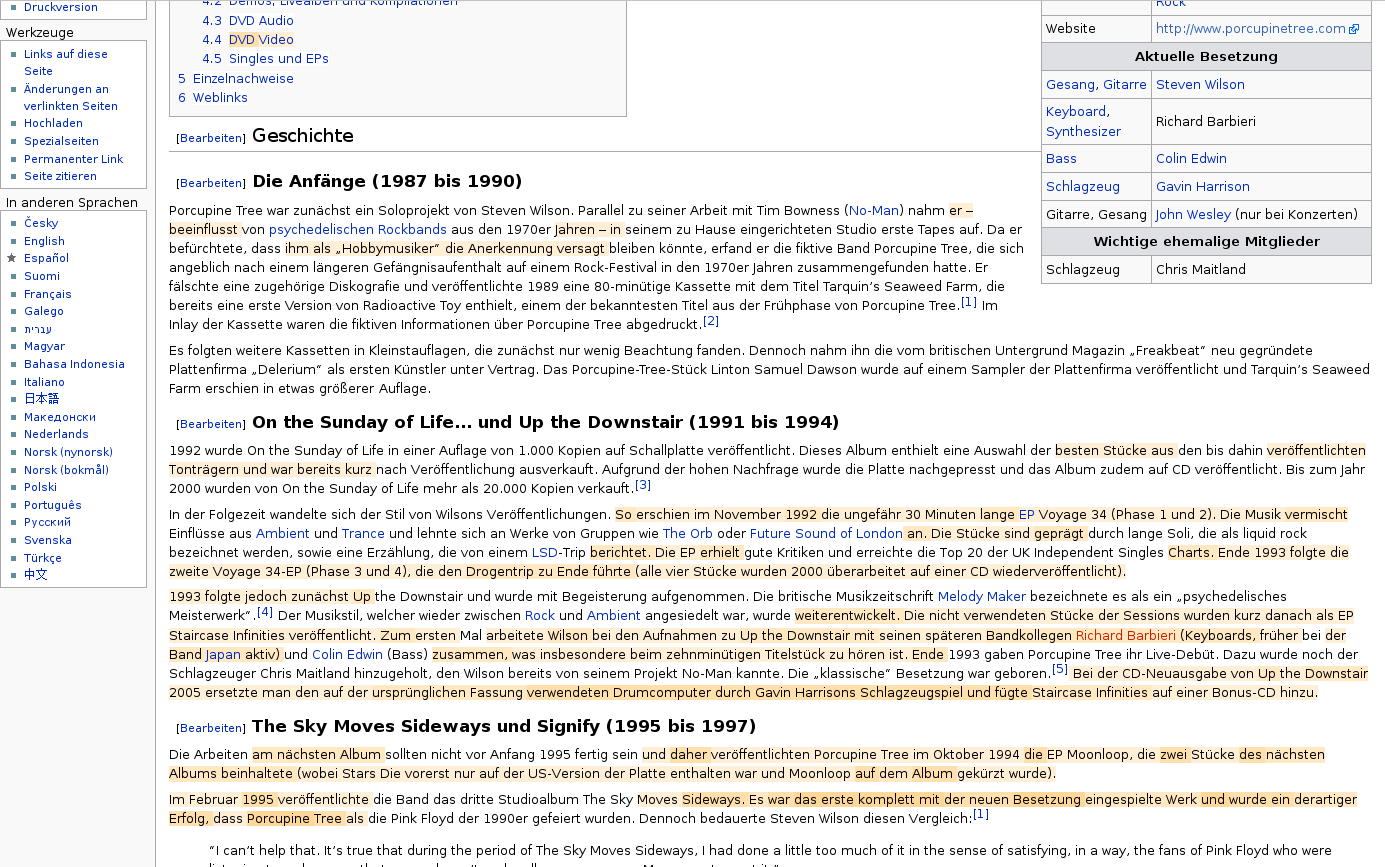
\includegraphics[width=0.8\textwidth,clip=true,resolution=300]{img/wikitrust.png}
         \caption{Wikitrust in action (2011)}
         \label{fig:wikitrust}
       \end{figure}

       \cite{Lucassen2011} Evaluating Wikitrust
       \cite{Lucassen2010} Trust in Wikipedia (how many links)
       

        %%%%%%%%%%%%%%%%%%%%%%%%%%%%%%%%%%%%%%%%%%%%%%%%%%%%%%%%%%%%
        %%
        %% CONCLUSIONS
        %%
        %%%%%%%%%%%%%%%%%%%%%%%%%%%%%%%%%%%%%%%%%%%%%%%%%%%%%%%%%%%%

        \section{Conclusions}
        Now we have reviewed the existing work, we will begin to
        outline our intentions. Here we discuss the assumptions that
        we make about our data, our intentions with regards to
        analysing that data, and the metrics by which we will regard
        each contribution.

        %% ASSUMPTIONS
        \subsubsection*{Assumptions}
        \begin{itemize}
          \item \textbf{We assume that the final, or 'target' article
            is of good quality.} There are many studies which concern
            themselves with verifying the accuracy and quality of
            Wikipedia articles. In this study we are specifically
            concerned with the quality of contribution, i.e. the
            quality of text within the article, relative to the domain
            of the article. The quality of the article itself is a
            moot point.
          \item \textbf{We assume the article is well-formed.} As much
            as we do not concern ourselves with article accuracy, we
            also assume that the Wikipedia markup is also
            well-formed. We may also eventually check whether links
            are invalid, but for the moment we assume that they are.
          \item \textbf{We make no distinction between humans, bots
            and anonymous editors.}
        \end{itemize}
        
        %%WEIGHTING BY MARKUP
        \subsubsection*{Weighting contribution by markup}
        Given the extesive research regarding which features of a
        wikipedia article are most important, we may define the
        following features to have more weight than standard text from
        the outset:
        \begin{itemize}
          \item Links
          \item Images
          \item Equations
        \end{itemize}

        We may either preprocess the text to identify the each of
        these different flavours of text by their Wikipedia mark-up
        conventions, or we may be able to more fluently work them into
        the main difference algorithm, raising and lowering flags
        during runtime.

        %%RESTRUCTURING
        \subsubsection*{Awarding restructuring}
        It has been found that, even in the most accurate articles,
        that the structure of Wikipedia article can be
        weak.\cite{Giles2005} We should award attempts to reorganize
        articles. We 
        
        %%DENSITY
        \subsubsection*{Awarding the dense edits}
        We should give extra reward to the density of the
        changes. For example, if we have a set of the indexes of an
        edit operation as $\{op_0,op_1,op_2,\dots, op_n\}$, where
        $op_i$ is the index of the $i$th operation, then we may
        evaluate it's density with a standard deviation of the edit
        itself, $\sigma_{ed}$, multiplied by the span of the edit
        itself in context of the wider article, and some weighting
        factor k. Something along the lines of:

        $$ed_{density} = k\bullet\frac{(op_n - op_0)\sigma_{ed}}{|v|}$$ 
        %% $\sigma_{ed} = \sqrt{\frac{\sum\limits_{i = 1}^{n}(op_i -
        %%   \overline{op})^2}{|op| - 1}}$\\

        where $|v_{ed}|$ is the overall length of resultant version. By
        implementing this carefully, we may achieve a gradient of
        weighting, with a lower weight values for things like
        spell-checks, and higher values for whole-paragraph changes.

        %% UNDONE OPERATIONS
        \subsection*{Undone and partially undone operations}
        We consider three different ways of classifying an edit as
        valueless, or partially valueless. Two ways of classifying
        these kinds of edit are found in previous research, and are
        covered in the figure below:

        \begin{figure}[H]
          \centering
          \begin{tikzpicture}
            \matrix (m) [matrix of math nodes, row sep=4em, column
              sep=4em] { & v_i & \\ v_{i-1} & & v_{i+1}\\ };
            \path[-stealth] (m-2-1) edge node [left]
                 {$ed(v_{i-1},v_i)$} (m-1-2) edge node [below]
                 {$ed(v_{i-1},v_{i+1})$} (m-2-3) (m-1-2) edge node
                 [right] {$ed(v_i,v_{i+1})$} (m-2-3); 
          \end{tikzpicture}\\
          a) if $ed(v_{i-1},v_i) < ed(v_{i-1},v_i) +
          ed(v_{i},v_{i+1})$, then $ed(v_{i-1},v_i)$ has been
          partially undone.\\ b) if $ed(v_{i-1},v_{i+1}) = 0$
          ($v_{i-1} = v_{i+1}$), then $ed(v_{i-1},v_i)$ has been
          completely undone.
          \caption{Diagram showing identification of apartially or
            completely undone edit}
          \label{fig:undo}
        \end{figure}

        We identify immediately undone or partially undone edits
        according to edit distance, as layed out in Adler et
        al\cite{Adler2007}. The triangle represents three consecutive
        revisions, and the arrows are the edit operations that
        transform one to another. By calculating the edit distance
        between $v_{i-1}$ and $v_{i+1}$ we may characterise a longer
        history of revisions than usual, and use that context in order
        to re-characterise the edits it encompasses. In the figure
        above, case $a$ describes $v_i$ as a 'diversion'. If $v_{i-1}$
        can be transformed into $v_{i+1}$ with less operations than
        the two edits that actually bridged that gap, then perhaps
        some of the edits in $v_{i-1} \rightarrow v_i$ were
        unnecessary, and undone by $v_{i+1}$. In this case, we may
          punish the edit $v_{i-1} \rightarrow v_i$ (for the
          diversion), reward $v_{i} \rightarrow v_{i+1}$, or
          both. Case $b$ is an extreme version of $a$ - the texts
          $v_{i-1}$ and $v_{i+1}$ are identical, so the changes in
            $v_i$ must have been completely, and immediately,
            undone. These reverts are common in Wikipedia edit
            practice.\cite{wiki-revert}

        These reverts, however, are limited in their scope. Although
        the system may easily be extended to cover larger spans of
        history, to consider all nodes in a history would require the
        edit-distance computation of many version pairs. I propose a
        different, more efficient way of characterising redundant
        entries in terms of longer history spans. The studies, mentioned
        above, that graph aim to graph a Wikipedia revision history,
        hint at a possible method of characterising redundant material
        in terms of a much larger time-frame. Again, we may utilise
        the fact taht we have take one article to be the ultimate
        destination of all previous edits. 

        Perhaps we may graph the entirety of a wikipedia's revision
        history in terms of the edit distance from this final version,
        thus:

        \begin{figure}[H]
          \centering
          \pgfplotsset{width=0.5\textwidth}
          \begin{tikzpicture}
            \begin{axis}[
                title={Dummy revision history},
                ylabel={edit distance from final version},
                xlabel={revision ID},
              ]
              \addplot table {dat/dummy_history.dat};
            \end{axis}
          \end{tikzpicture}
          \label{fig:dummy_history}
        \end{figure}
        
        Each point represents a different version, and each line
        represents the the edit-distance between each version. Given
        this information, we may be able to disregard some information
        by only considering revisions that bring us closer to the
        final version. They appear on this graph as lines with a
        negative gradient; those with a positive gradient take us
        further away from the final version:

        \begin{figure}[H]
          \centering
          \pgfplotsset{width=0.5\textwidth}
          \begin{tikzpicture}
            \begin{axis}[
                title={Dummy revision history},
                ylabel={edit distance from final version},
                xlabel={revision ID},
              ]
              \addplot [blue] table {dat/dummy1.dat};
              \addplot [red] table {dat/dummy2.dat};
              \addplot [blue] table {dat/dummy3.dat};
              \addplot [blue, only marks] table {dat/dummy4.dat};
            \end{axis}
          \end{tikzpicture}
          \label{fig:dummy_optimisation_1}
        \end{figure}

        We may ignore the lines with a positive gradient (the two
        red lines). This is simple to implement. Given a version
        $v_i$, having computed it's immediate edit distance
        $ed(v_{i-1},v_i)$, and it's edit distance from the final
        version, $ed_{final_i}$, we know our next computation must be
        $ed(v_{j-1},ed_j)$, such that $j$ is the smallest number that
        satisfies the qualities $j > i$ and $ed_{final_j} <
        ed_{final_{j-1}}$. 

        Another possible version would be to disregard all edit
        distances that, at any point, lie between two versions that
        are further away from final version than the version
        currently being considered.

        \begin{figure}[H]
          \centering
          \pgfplotsset{width=0.5\textwidth}
          \begin{tikzpicture}
            \begin{axis}[
                title={Dummy revision history},
                ylabel={edit distance from final version},
                xlabel={revision ID},
              ]
              \addplot [blue] table {dat/dummy1.dat};
              \addplot [red] table {dat/dummy5.dat};
              \addplot [blue] table {dat/dummy6.dat};
              \addplot [blue, only marks] table {dat/dummy4.dat};
              \fill [orange!25,fill opacity=0.5] (axis cs:4,13) rectangle (rel axis
              cs:1,1);
              \addplot[red,dashed,update limits=false] 
	      coordinates {(-2,13) (14,13)};
              \addplot[red,dashed,update limits=false] 
	      coordinates {(4,13) (4,22)};
            \end{axis}
          \end{tikzpicture}
          \label{fig:dummy_optimisation_2}
        \end{figure}
        
        The green area shows the area in which we look to find
        $v_j$. Here, after considering $v_i$, we move to $v_j$, such
        that $j$ is the smallest number that satisfies to qualities $j
        > i$ and $ed_{final_j} < ed_{final_i}$. In the graph above we
        move from (4,13) to (8,12). It is worth stating here that
        always compute $ed(v_{j-1}, v_j)$, not necessarily
        $ed(v_i,v_j)$. We will look into the pros and cons of these
        different strategies further into the project.

        \subsection*{Possible extensions}
        \subsubsection*{Visualisation}
        Given that we are distributing wealth according to a series of
        weight factors, it may be useful to devise a system that
        visualises how these weight factors affect the
        distribution. This would be a matter of expressing the final
        'score' in terms of these variables, and producing some
        interactive graphs. We will look into the viability of this
        extension further into the project.
        
        \subsubsection*{Data}
        Current intentions are to approach the data on an
        article-by-article basis, grabbing a particular version and
        tracing its history backwards. We grab the pages using HTTP
        requests, as described earlier (see page
        \ref{wikipedia-api}). We could, however, download Wikipedia in
        its entirety. The entire site is compressed and dumped
        monthly, and the dumps are free to download.\cite{wiki-dump}

        \subsubsection*{Further analysis}
        Given the over-arching nature of Wikis, it may be possible to
        derive other information about the articles we
        study. By-products of this study include various ways to
        visualise the histories of different articles, and
        comprehensive storage of various dimensions of Wikipedia
        artefacts and agents. We may be able compare and contrast
        different categories of article, or editor. It would be
        interesting to contrast the actions of humans, and
        bots,\footnote{It has been noted that there are around 700
          bots registered on Wikipedia (as of 2014). Though not all of
          them make edits, those that do are very prolific, and are
          known to reverse malicious submisions in a matter of
          seconds.\cite{wiki-bots}\cite{bbc-bots}}, and perhaps look
        at the nature of edits made by different groups of editors.

        %%%%%%%%%%%%%%%%%%%% FIND ROOM
        
        It may be worth Perhaps we can examine more about what
        we may find out about the articles. Cite other studies Lih's
        2004 study of articles immediately after they have been cited
        in the press\cite{Lih2004}, and Metyan's 2012 use of the site
        to predict box-office success \cite{Mestyan2012}. Lieberman
        worked out their locale.\cite{Lieberman2009}:

        %%%%%%%%%%%%%%%%%%%% FIND ROOM

        \subsubsection*{Further subjects}
        The project may well extend to subjects beyond Wikipedia. A
        github project, for instance may be of interest in further
        study. We may begin to look into software metrics, such as
        Cyclomatic Complexity, which measures code flow complexity
        according to its logical operators,\cite{McCabe1976} as well
        as others, and figure out ways of regarding non-linear
        revision histories.

        \begin{enumerate}
          \item peaks in activity (rate of levenshtein distance... may
            have to be in a log graph...)
          \item 
        \end{enumerate}

        PREDIFINED / NOT-PREDEFINED ideas of quality. look for when
        the the article levels off? And do this by DATE rather than
        REVISION. We may assume that pageviews are more
        well-distributed than revisions

        summarize major contributions (which do we care about?)
        evaluate your current position point out any flaw in
        methodology/research/contradictions are there any gaps in the
        area which you will cover in your researchq?  How will you
        integrate sources you have mentioned into your dissertation?
        Point out any areas for further study


        \section{Progress report}
        One python scraper

        One simple python levenshtein distance
        - Have defined a format for storing edit operation: array of
        tuples. Will work on extending this. MAy have to be a
        dictionary to deal with flags
        - Have not yet implemented other versions of the algorithm,
        that is next step

        One class combining both is in progress.
        
        \clearpage
        \printbibheading[heading=bibintoc,title={References}]
        \printbibliography
        %% \printbibliography[keyword=wiki,heading=subbibliography,title={Wikipedia}]
        %% \printbibliography[keyword=edit,heading=subbibliography,title={Edit
        %%     distance}]
        
        
        \clearpage
        \begin{appendices}
          \section{Appendix A: Code progress}
          \subsection{Python class for scraping a Wikipedia article's
            revision history}
          \label{wiki-scrape}
          The following code is a first draft of a class which incrementally
          traces, parses, and stores the revision history of select articles. It
          chooses random articles up to a maximum amount of articles unless an
          article (or articles) are specified. It traces the entire
          discoverable\footnote{Using the Wikipedia API, articles can either be
            traced back to their origin (revision parent ID = 0), or to the
            point at which a loop is found in the revision history - this
            usually happens with older articles.} history of the, unless a
          specific depth is specified by the user.
          
          The class already yields workable data, but here is some immediate
          further work for this code:
          \begin{itemize}
          \item Allow the user to specify timeframe
          \item Allow for integration with a postgres database (at the moment
            the code saves the data in CSV format).
          \end{itemize}
          
          This code is an extension to an existing wikipedia API class for
          python (which did not provide the features we need
          here).\cite{python-wikipedia}
          
          \lstinputlisting[language=Python,frame=single]{../code/wikiScraper/WikiRevisionScrape.py}
          \subsection{Example output}
          \fvset{frame=single}
          \VerbatimInput{../code/wikiScraper/output.txt}
          
          \clearpage
          \section{Appendix B: Python Levenshtein distance implementation}
          \label{levenshtein-implement}
          This Python class gives a basic implementation of
          Levenshtein distance. To compare strings $x$ and $y$ both
          its time and space complexity is
          ${\Theta}log(|x|{\bullet}|y|)$.

          The class is instantiated with the twwo strings, or files,
          it is to compare. Methods can then be accessed in order to
          examine the distance between the provided strings. The class
          provides command-line visualisations of the data --- it can
          print out its table of computations, as well as instructions
          on how to transform one into the other. Please see the
          exmple output below. It does not currently give any
          information about optimal alignment, although information
          about this alignment is found in the table.
          \subsection{Code}
          \lstinputlisting[language=Python,frame=single]{../code/lshtein/basic/LevDistBasic.py}
          \subsection{Example output}
          \fvset{frame=single}
          \VerbatimInput{../code/lshtein/basic/output.txt}
        \end{appendices}
        
\end{document}
